% =====================================
\chapter{Qu'est-ce qu'un algorithme ?}
% =====================================

\begin{center}
	\textit{«~L'algorithmique est le permis de conduire de l'informatique.
	Sans elle, il n'est pas concevable d'exploiter sans risque un ordinateur.~»
	\footnote{[CORMEN e.a., Algorithmique, Paris, Edit. Dunod, 2010, (Cours, 
	exercices et problèmes), p. V] }}
\end{center}

\marginicon{objectif}
Ce chapitre a pour but de vous faire comprendre ce
qu'est un \textbf{algorithme} et à quel moment de
l'\textbf{activité de programmation} il intervient. 
Nous tenterons de préciser la différence entre un algorithme 
et un \textbf{programme}.

Il situe, enfin, le cours de \textit{logique et techniques de
programmation} dans l’ensemble des cours donnés dans le baccalauréat et
en trace les lignes principales.

\section{La notion de problème}

	\subsection{Préliminaires~: utilité de l’ordinateur}
	
		L’ordinateur est une machine. Mais une machine intéressante dans la
		mesure où elle est destinée d’une part, à nous décharger d’une
		multitude de tâches peu valorisantes, rébarbatives telles que le
		travail administratif répétitif, mais surtout parce qu’elle est capable
		de nous aider, voire nous remplacer, dans des tâches plus ardues qu’il
		nous serait impossible de résoudre sans son existence (conquête
		spatiale, prévision météorologique, jeux vidéo, ...).
		
		En première approche, nous pourrions dire que l’ordinateur est destiné à
		nous remplacer, à faire à notre place (plus rapidement et probablement
		avec moins d’erreurs) un travail nécessaire à la résolution de
		\textbf{problèmes} auxquels nous devons faire face. Attention ! Il
		s’agit bien de résoudre des \textit{problèmes} et non des mystères
		(celui de l’existence, par exemple). Il faut que la question à laquelle
		on souhaite répondre soit \textbf{accessible à la raison}.

	\subsection{Poser le problème}
	
		Un préalable à l’activité de résolution d’un problème est bien de
		\textbf{définir} d’abord quel est le problème posé, en quoi il consiste
		exactement ; par exemple, faire un baba au rhum, réussir une année
		d’études, résoudre une équation mathématique\dots
		
		Un problème bien posé doit mentionner l’\textbf{objectif à atteindre},
		c’est-à-dire la situation d’arrivée, le but escompté, le résultat
		attendu. Généralement, tout problème se définit d’abord explicitement
		par ce que l’on souhaite obtenir.
		
		La formulation d’un problème ne serait pas complète sans la connaissance
		des \textbf{données du problème} et \textbf{du cadre dans lequel se
		pose le problème~:} de quoi dispose-t-on, quelles sont les hypothèses
		de base, quelle est la situation de départ ? Faire un baba au rhum est
		un problème tout à fait différent s’il faut le faire en plein désert ou
		dans une cuisine super équipée! D’ailleurs, dans certains cas, la
		première phase de la résolution d’un problème consiste à mettre à sa
		disposition les éléments nécessaires à sa résolution~: dans notre
		exemple, ce serait se procurer les ingrédients et les ustensiles de
		cuisine.
	
		Un problème ne sera véritablement bien spécifié que s’il s’inscrit dans
		le schéma suivant~:
		
		% Voir si j'en fait un environnement.
		\begin{center}
		\begin{Ovalbox}
		{\textstyleMotCl{étant donné} [les données] \textstyleMotCl{on demande} [l’objectif]}
		\end{Ovalbox}
		\end{center}
	
		Parfois, la première étape dans la résolution d’un problème est de
		préciser ce problème à partir d’un énoncé flou~: il ne s’agit pas
		nécessairement d’un travail facile !

		\begin{Emphase}[exercice]{Exercice~: Un problème flou}
			Soit le problème suivant~: «~Calculer la moyenne de nombres entiers.~».
			\\Qu'est-ce qui vous parait flou dans cet énoncé ?
		\end{Emphase}

		Une fois le problème correctement posé, on passe à la recherche et la
		description d’une \textbf{méthode de résolution}, afin de savoir
		comment faire pour atteindre l’objectif demandé à partir de ce qui est
		donné. Le \textbf{nom} donné à une méthode de résolution varie en
		fonction du cadre dans lequel se pose le problème~: \textit{façon de
		procéder, mode d’emploi, marche à suivre, guide, patron, modèle,
		recette de cuisine, méthode ou plan de travail, algorithme
		mathématique, programme, directives d’utilisation,...}

\section{Procédure de résolution}

	Une \textbf{procédure de résolution }est une description en termes
	compréhensibles par l'exécutant de la \textbf{marche à
	suivre} pour résoudre un problème donné.
	
	On trouve beaucoup d'exemples dans la vie courante~:
	recette de cuisine, mode d’emploi d’un GSM, description d’un
	itinéraire, plan de montage d’un jeu de construction, etc. Il est clair
	qu’il y a une infinité de rédactions possibles de ces différentes
	marches à suivre. Certaines pourraient être plus précises que d’autres,
	d’autres par contre pourraient s’avérer exagérément explicatives.
	
	Des différents exemples de procédures de résolution se dégagent les
	caractéristiques suivantes:

	\begin{liste}
	\item toutes ont un \textbf{nom}
	\item elles s’expriment dans un \textbf{langage}
		(français, anglais, dessins\dots)
	\item l’ensemble de la procédure consiste 
		en une \textbf{série chronologique}
		d’instructions ou de phrases (parfois numérotées)
	\item une instruction se caractérise par un ordre, 
		une action à accomplir,
		une \textbf{opération} à exécuter sur les \textbf{données} du problème
	\item certaines phrases justifient ou expliquent ce qui se passe~: 
		ce sont des \textbf{commentaires}.
	\end{liste}

	On pourra donc définir, en première approche, une procédure de
	résolution comme un texte, écrit dans un certain langage, qui décrit
	une suite d’actions à exécuter dans un ordre précis, ces actions
	opérant sur des objets issus des données du problème.

	\subsection{Chronologie des opérations}

		Pour ce qui concerne l’ordinateur, le travail d’exécution d’une marche à
		suivre est impérativement \textbf{séquentiel}. C’est-à-dire que les
		instructions d’une procédure de résolution sont exécutées \textbf{une
		et une seule fois} dans l’ordre où elles apparaissent dans le code.
		Cependant certains artifices d’écriture permettent de \textbf{répéter}
		l’exécution d’opérations ou de la \textbf{conditionner}
		(c'est-à-dire de choisir si
		l'exécution aura lieu oui ou non en fonction de la
		réalisation d'une condition).

	\subsection{Les opérations élémentaires}


		Dans la description d’une marche à suivre, la plupart des opérations
		sont introduites par un \textbf{verbe
		}(\textit{remplir,}\textbf{\textit{ }}\textit{verser, prendre, peler},
		etc). L’exécutant ne pourra exécuter une action que si il la comprend~:
		cette action doit, pour lui, être une action élémentaire, une action
		qu’il peut réaliser sans qu’on ne doive lui donner des explications
		complémentaires. Ce genre d’opération élémentaire est appelée
		\textbf{primitive}.
		
		Ce concept est évidement relatif à ce qu’un exécutant est capable de
		réaliser. Cette capacité, il la possède d’abord parce qu’il est
		\textbf{construit} d’une certaine façon (capacité innée). Ensuite parce
		que, par construction aussi, il est doté d’une faculté
		d’\textbf{apprentissage} lui permettant d’assimiler, petit à petit, des
		procédures non élémentaires qu’il exécute souvent. Une opération non
		élémentaire pourra devenir une primitive un peu plus tard.
		
		%Enfin, il est tout à fait possible que l’exécutant s’adjoigne un
		%auxiliaire, un \textbf{aide}, lui permettant de traduire une opération
		%non élémentaire (qu’il ne comprend donc pas) en une suite d’opérations
		%primitives.

	\subsection{Les opérations bien définies}

		Il arrive de trouver dans certaines marches à suivre des opérations qui
		peuvent dépendre d’une certaine manière de l’appréciation de
		l’exécutant. Par exemple, dans une recette de cuisine on pourrait lire
		: \textit{ajouter }\textbf{\textit{une pincée }}\textit{de vinaigre,
		saler et poivrer }\textbf{\textit{à volonté}}\textit{, laisser cuire
		une }\textbf{\textit{bonne}}\textit{ heure dans un four
		}\textbf{\textit{bien}}\textit{ chaud, etc.}
		
		Des instructions floues de ce genre sont dangereuses à faire figurer
		dans une bonne marche à suivre car elles font appel à une appréciation
		arbitraire de l'exécutant. Le résultat obtenu risque
		d’être imprévisible d’une exécution à l’autre. De plus, les termes du
		type \textit{environ, beaucoup, pas trop} et \textit{à peu près }sont
		intraduisibles et proscrites au niveau d’un langage informatique
		!\footnote{Le lecteur intéressé découvrira dans la littérature
		spécialisée que même les procédures de génération de nombres aléatoires
		sont elles aussi issues d’algorithmes mathématiques tout à fait
		déterminés.}
		
		Une \textbf{opération bien définie} est donc une opération débarrassée
		de tout vocabulaire flou et dont le résultat est \textbf{entièrement
		prévisible}. Des versions «~bien définies~» des exemples ci-dessus
		pourraient être~: \textit{ajouter 2 cl de vinaigre, ajouter 5 g de sel
		et 1 g de poivre, laisser cuire 65 minutes dans un four chauffé à
		220°C, etc.}

		Afin de mettre en évidence la difficulté d'écrire une
		marche à suivre claire et non ambigüe, on vous propose
		l'expérience suivant.

		\begin{Emphase}[exercice]{Expérience~: Le dessin}

			Cette expérience s'effectue en groupe.
			Le but est de faire un dessin et de permettre à une autre personne, qui
			ne l'a pas vu, de le reproduire fidèlement, au travers
			d'une «~marche à suivre~».

			\begin{enumerate}
			\item
				Chaque personne prend une feuille de papier et 
				y dessine quelque chose en quelques traits précis. 
				Le dessin ne doit pas être trop compliqué; 
				on ne teste pas ici vos talents de dessinateur ! 
				(ça peut-être une maison, une voiture, ...)
			\item
				Sur une \textbf{autre} feuille de papier, 
				chacun rédige des instructions permettant de 
				reproduire fidèlement son propre dessin. 
				Attention ! Il est important de ne
				\textbf{jamais faire référence à la signification du dessin}. 
				Ainsi, on peut écrire~: «~dessine un rond~» 
				mais certainement pas~: «~dessine une roue~».
			\item
				Chacun cache à présent son propre dessin et échange 
				sa feuille d'instructions avec celle de quelqu'un d'autre.
			\item
				Chacun s'efforce ensuite de reproduire le dessin d'un autre 
				en suivant \textbf{scrupuleusement} les instructions indiquées 
				sur la feuille reçue en échange, \textbf{sans tenter
				d'initiative} (par exemple en croyant avoir compris ce
				qu'il faut dessiner).
			\item
				Nous examinerons enfin les différences entre l'original et 
				la reproduction et nous tenterons de comprendre pourquoi 
				elles se sont produites (par imprécision des instructions ou
				par mauvaise interprétation de celles-ci par le dessinateur...)
			\end{enumerate}

		\end{Emphase}

\bigskip
		\marginicon{reflexion}
		Quelles réflexions cette expérience vous inspire-t-elle ?
		Quelle analogie voyez-vous avec une marche à suivre donnée à un
		ordinateur ?

		Dans cette expérience, nous imposons que la «~marche à suivre~» ne mentionne
		aucun mot expliquant le sens du dessin (mettre «~rond~» et pas «~roue~»
		par exemple). Pourquoi, à votre avis, avons-nous imposé cette
		contrainte ?

	\subsection{Opérations soumises à une condition}

		En français, l’utilisation de conjonctions ou locutions conjonctives du
		type \textit{si}\textit{, selon que, }\textit{au cas où, }etc\dots
		présuppose la possibilité de ne pas exécuter certaines opérations en
		fonction de certains événements. D’une exécution à l’autre de
		l’entièreté de la procédure, certaines de ses parties seront ou non
		exécutées.
		
		\textbf{Exemple~:} Si la viande est surgelée, la décongeler à
		l'aide du four à micro-onde.

	\subsection{Opérations à répéter}

		De la même manière, il est possible d’exprimer en français une exécution
		répétitive d’opérations en utilisant les mots \textit{tous},
		\textit{chaque}, \textit{tant que}, \textit{jusqu’à ce que},
		\textit{chaque fois que}, \textit{aussi longtemps que}, 
		\textit{faire x fois},\dots 
		
		Dans certains cas, le nombre de répétitions est connu à l’avance
		(\textit{répéter 10 fois}) ou déterminé par une durée (\textit{faire
		cuire pendant 30 minutes}) et dans d’autres cas il est inconnu.
		Dans ce cas, la fin de la période
		de répétition d’un bloc d’opérations dépend alors de la réalisation
		d’une condition ((\textit{lancer le dé jusqu'à ce
		qu'il tombe sur 6}), \dots, \textit{faire cuire
		jusqu’à évaporation complète}\dots). C’est ici que réside le danger de
		boucle infinie, due à une mauvaise formulation de la condition d’arrêt.
		Par exemple~: \textit{lancer le dé jusqu’à ce que le point 
		obtenu soit 7}\dots Bien sûr, un humain doté d'intelligence 
		comprend que la condition est impossible à réaliser, mais un robot 
		appliquant cette directive à la lettre lancera le dé 
		perpétuellement\dots

	\subsection{À propos des données}

		Les types d’objets figurant dans les diverses procédures de résolution
		sont fonction du cadre dans lequel s’inscrivent ces procédures, du
		domaine d’application de ces marches à suivre. Par exemple, pour une
		recette de cuisine, ce sont les ingrédients. Pour un jeu de
		construction ce sont les briques.
		
		L'ordinateur, quant à lui, manipule principalement
		des données numériques et textuelles. 
		Nous verrons plus tard comment on
		peut combiner ces données élémentaires pour obtenir 
		des données plus complexes.

\section{Algorithmes informatiques}

	Notre but étant de faire de l’informatique, il convient de restreindre
	notre étude à des notions plus précises, plus spécialisées, gravitant
	autour de la notion de \textit{traitement automatique de
	l’information}.

	\subsection{Algorithme}

		Un algorithme appartient au vaste ensemble des \textit{marches à
		suivre.}

		\marginicon{definition}
		\textbf{Algorithme}~: Procédure de résolution d'un problème 
		ou d'un ensemble de problèmes de même type contenant des opérations
		bien définies portant sur des informations, s’exprimant dans une
		séquence définie sans ambigüité, destinée à être traduite dans 
		un langage de programmation.
	
		Comme toute marche à suivre, un algorithme doit s’exprimer dans un
		certain langage~: à priori le langage naturel , mais il y a d’autres
		possibilités~: ordinogramme, arbre programmatique, pseudo-code ou LDA
		(langage de description d’algorithmes) que nous allons utiliser dans le
		cadre de ce cours.

	\subsection{Programme}

		\marginicon{definition}
		Un \textbf{programme} n’est rien d’autre que la représentation d’un
		algorithme dans un langage plus technique compris par 
		un ordinateur (par exemple~:
		Assembleur, Cobol, Java, 
		C++, ...). Ce type de langage est appelé \textbf{langage de
		programmation}.
		
		Écrire un programme correct suppose donc la parfaite connaissance du
		langage de programmation et de sa \textbf{syntaxe}, qui est en quelque
		sorte la grammaire du langage. Mais ce n’est pas suffisant ! Puisque le
		programme est la représentation d’un algorithme, il faut que celui-ci
		soit correct pour que le programme le soit. Un programme correct
		résulte donc d’une démarche logique correcte (algorithme correct) et de
		la connaissance de la syntaxe d’un langage de programmation.
		
		Il est donc indispensable d’élaborer des algorithmes corrects avant
		d’espérer concevoir des programmes corrects.

	\subsection{Les constituants principaux de l’ordinateur}

		Les constituants d’un ordinateur se divisent en \textbf{hardware}
		(matériel) et \textbf{software d’exploitation} (logiciel).
		
		Le \textbf{hardware} est constitué de l’ordinateur proprement dit et
		regroupe les entités suivantes~:

		\begin{liste}
		\item
			\textbf{l’organe de contrôle~:} c’est le cerveau de
			l'ordinateur. Il est l’organisateur, le contrôleur
			suprême de l’ensemble. Il assume l’enchainement des opérations
			élémentaires. Il s’occupe également d’organiser l’exécution effective
			de ces opérations élémentaires reprises dans les programmes.
		\item
			\textbf{l’organe de calcul~:} c’est le calculateur où ont lieu les
			opérations arithmétiques ou logiques. Avec l’organe de contrôle, il
			constitue le \textbf{processeur} ou \textbf{unité centrale}.
		\item
			\textbf{la mémoire centrale~:} dispositif permettant de mémoriser,
			pendant le temps nécessaire à l’exécution, les programmes et certaines
			données pour ces programmes.
		\item
			\textbf{les unités d’échange avec l’extérieur~:} dispositifs permettant
			à l’ordinateur de recevoir des informations de l’extérieur (unités de
			lecture telles que clavier, souris, écran tactile,...) ou de
			communiquer des informations vers l’extérieur (unités d’écriture telles
			que écran, imprimantes, signaux sonores, \dots).
		\item
			\textbf{les unités de conservation à long terme~:} ce sont les mémoires
			auxiliaires (disques durs, CD ou DVD de données, clés USB,...) sur
			lesquels sont conservées les procédures (programmes) ou les
			informations résidentes dont le volume ou la fréquence d’utilisation ne
			justifient pas la conservation permanente en mémoire centrale.
		\end{liste}
		
		Le \textbf{software d’exploitation} est l’ensemble des procédures
		(programmes) s’occupant de la gestion du fonctionnement d’un système
		informatique et de la gestion de l’ensemble des ressources de ce
		système (le matériel – les programmes – les données). Il contient
		notamment des logiciels de traduction permettant d’obtenir un programme
		écrit en langage machine (langage technique qui est le seul que
		l’ordinateur peut comprendre directement, c’est-à-dire exécuter) à
		partir d’un programme écrit en langage de programmation plus ou moins
		«~évolué~» (c’est-à-dire plus ou moins proche du langage naturel).

	\subsection{Exécution d'un programme}

		Isolons (en les simplifiant) deux constituants essentiels de
		l'ordinateur afin de comprendre ce qui se passe quand
		un ordinateur exécute un programme. D'une part, la
		mémoire contient le programme et les données manipulées par ce
		programme. D'autre part, le processeur va «~exécuter~»
		ce programme.

		\begin{tabular}{m{0.48\linewidth}m{0.48\linewidth}}
			\begin{center}
			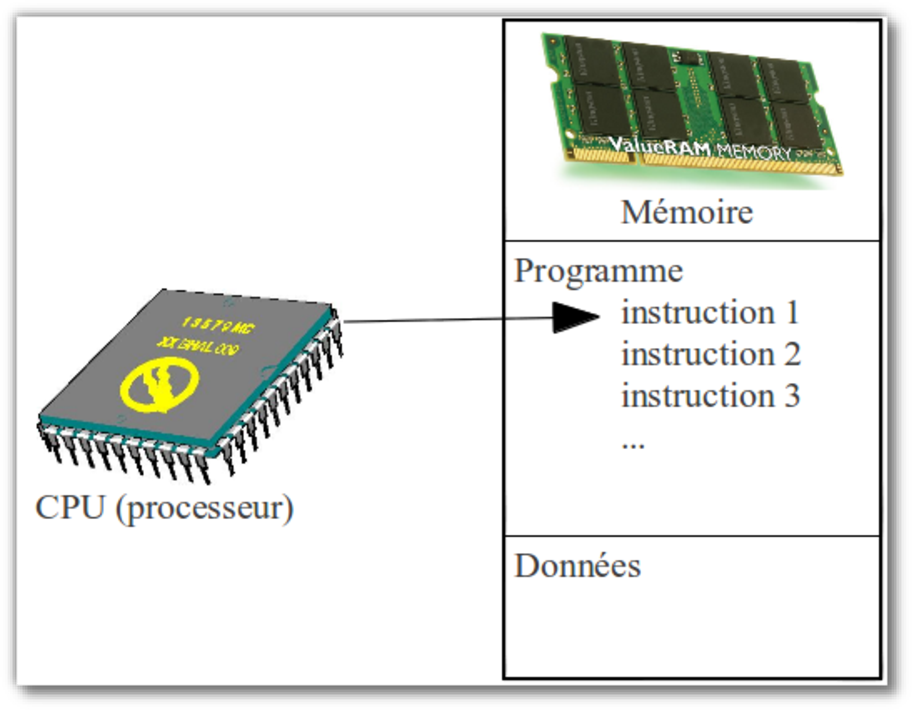
\includegraphics[width=0.45\textwidth]{image/intro-schema-ordi}
			\end{center}
		&
			\textbf{Comment fonctionne le processeur ?}
	
			De façon très simplifiée, on passe par les étapes suivantes~:
	
			\medskip
			\begin{flushleft}
			\begin{enumerate}
			\item Le processeur lit l'instruction courante.
			\item Il exécute cette instruction. Cela peut amener à manipuler les données.
			\item L'instruction suivante devient l'instruction courante.
			\item On revient au point 1
			\end{enumerate}
			\end{flushleft}
		\\
		\end{tabular}

		On voit qu'il s'agit d'un travail
		automatique ne laissant aucune place à l'initiative !

\section{Les phases d'élaboration d'un programme}

	Voyons pour résumer un schéma \textbf{simplifié} des phases par
	lesquelles il faut passer quand on développe un programme.

	\begin{tabular}{m{0.25\linewidth}m{0.72\linewidth}}
	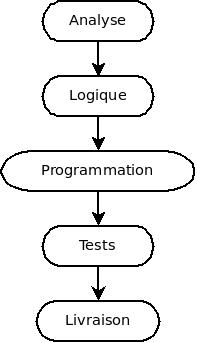
\includegraphics[width=3.5cm]{image/intro-phases-develop}
	&
	\begin{liste}
	\item 
		Lors de \textbf{l'analyse}, le problème doit être
		compris et clairement précisé. Vous aborderez cette phase dans le cours
		d'analyse.
	\item
		Une fois le problème analysé, et avant de passer à la phase de
		programmation, il faut réfléchir à l'\textbf{algorithme} qui va
		permettre	de résoudre le problème. C'est à cette phase précise
		que s'attache ce cours.
	\item
		On peut alors \textbf{programmer} cet algorithme dans le langage de
		programmation choisi. Vos cours de langage (Java, Cobol, 
		Assembleur, \dots) est dédié à cette phase.
	\item
		Vient ensuite la phase de \textbf{tests} qui ne manquera pas de montrer
		qu'il subsiste des problèmes qu'il
		faut encore corriger. (Vous aurez maintes fois
		l'occasion de vous en rendre compte lors des
		séances de laboratoire)
	\item
		Le produit sans bug (connu), peut être \textbf{mis en application}
		ou \textbf{livré} à la personne qui vous en a passé la commande.
	\end{liste}
	\\
	\end{tabular}
	
	Notons que ce processus n'est pas linéaire. À chaque
	phase, on pourra détecter des erreurs, imprécisions ou oublis des
	phases précédentes et revenir en arrière.

	\textbf{Pourquoi passer par la phase «~logique~» 
		et ne pas directement passer à la programmation ?}
	
	Voilà une question que vous ne manquerez pas de vous poser pendant votre
	apprentissage cette année. Apportons quelques éléments de réflexion.

	\begin{liste}
	\item
		Passer par une phase de «~logique~» permet de séparer deux difficultés~:
		quelle est la marche à suivre ? Et comment l'exprimer
		dans le langage de programmation choisi ? Le langage que nous allons
		utiliser en logique est plus souple et plus général que le langage Java
		par exemple (où il faut être précis au « ;~» près)
	\item
		De plus, un algorithme écrit facilite le dialogue dans une équipe de
		développement. «~J'ai écrit un algorithme pour
		résoudre le problème qui nous occupe. Qu'en
		pensez-vous ?~Pensez-vous qu'il est correct ?
		Avez-vous une meilleure idée ?». L'algorithme est plus adapté à la
		communication car plus lisible.
	\item
		Enfin, si la logique est écrite elle pourra facilement être traduite
		dans n'importe quel langage de programmation. La
		traduction d'un langage de programmation à un autre
		est un peu moins facile à cause des particularités propres à chaque
		langage.
	\end{liste}

	Bien sûr, cela n'a de sens que si le problème présente
	une réelle difficulté logique. Certains problèmes (en pratique,
	certaines parties de problèmes) sont suffisamment simples que pour être
	directement programmés. Mais qu'est-ce
	qu'un problème simple ? Cela va évidemment changer
	tout au long de votre apprentissage. Un problème qui vous paraitra
	difficile en début d'année vous paraitra (enfin, il
	faut l'espérer !) une évidence en fin
	d'année.

\section{Conclusion}

	L’informatisation de problèmes est un processus essentiellement
	dynamique, contenant des allées-venues constantes entre les différentes
	étapes. Codifier un algorithme dans un langage de programmation
	quelconque n’est certainement pas la phase la plus difficile de ce
	processus. Par contre, élaborer une démarche logique de résolution d’un
	problème est probablement plus complexe.
	
	Le but du cours de \textbf{logique et techniques de programmation} est
	double~:

	\begin{liste}
	\item
		essayer de définir une bonne démarche d’élaboration d’algorithmes
		(apprentissage de la \textbf{logique} de programmation);
	\item
		faire comprendre l’intérêt d’utiliser certaines méthodes ou
		\textbf{techniques} classiques qui ont fait leurs preuves.
	\end{liste}

	Le tout devrait avoir pour résultat l’élaboration de \textit{bons
	programmes}, c’est-à-dire \textit{des programmes dont il est facile de
	se persuader qu’ils sont corrects} et des programmes dont la
	maintenance est la plus aisée possible. Dans ce sens, ce cours se situe
	idéalement en aval d’un cours d’\textbf{analyse}, et en amont des cours
	de \textbf{langage de programmation}. Ceux-ci sont idéalement complétés
	par les notions de \textbf{système d’exploitation} et de
	\textbf{fichiers}.

	Afin d’envisager la résolution d’une multiplicité de problèmes prenant
	leur source dans des domaines différents, le contenu minimum de ce
	cours envisage l’étude des points suivants (dans le désordre)~:

	\begin{liste}
	\item 
		la représentation des algorithmes
	\item
		la programmation structurée
	\item
		la programmation procédurale~: les modules et 
		le passage de paramètres
	\item
		les bases de la programmation orientée objet
	\item
		la logique de traitement des fichiers séquentiels
	\item
		la logique de traitement des tableaux
	\item
		la résolution de problèmes récursifs
	\item
		la logique de traitement des structures de données particulières telles
		que listes, files d’attente, piles, arbres, graphes, tables de hachage,
		etc.
	\end{liste}

	Voilà bien un programme trop vaste pour une année d’étude, même pour un
	cours de 100 heures ! Un choix devra donc être fait et ce, en fonction
	de critères tels que la rapidité d’assimilation, l’intérêt des
	étudiants et les besoins exprimés pour des cours annexes. Les
	matières non traitées en 1\up{ère} année 
	seront étudiées au cours de logique de 2\up{ème} année.

\section{Références}
	
	On reprend ici une liste de livres et sites que vous pouvez consulter
	tout au long de votre apprentissage de
	l'algorithmique. Certaines références, plus
	spécifiques, seront fournies avec les chapitres qui les concernent.

	\begin{liste}
	\item 
		Alain Cardon et Christophe Dabancourt~: «~\textit{Initiation à
		l'algorithmique objet}~» aux éditions Eyrolles. ISBN
		2-212-09258-X
		\textit{Un ouvrage très clair sur l'algorithmique qui
		suit assez bien le cours de logique même si les notations sont un peu
		différentes.}
	\item
		Claude Delannoy~: «~\textit{Initiation à
		l'informatique}~» aux éditions Eyrolles. 
		ISBN 978-2212088724
		\textit{Un livre pédagogique adapté à un étudiant de première année.}
	\end{liste}
